\documentclass[a4paper, 12pt]{article}

\usepackage{listings}
\usepackage{color}
\usepackage[frenchb]{babel}
\usepackage[utf8]{inputenc}
\usepackage[T1]{fontenc}
\usepackage{lmodern}
\usepackage{graphicx}
% Numbers and units
\usepackage[squaren, Gray]{SIunits}
\usepackage{sistyle}
\usepackage[autolanguage]{numprint}
\usepackage{fullpage}
\usepackage{hyperref}
\usepackage{multirow}
\usepackage{xparse}
\usepackage{tikz}
\usepackage{enumitem}
\usepackage{amsmath}

\setlength{\parskip}{1em}
\usetikzlibrary{arrows, decorations.markings}

\newcommand\si[2]{\numprint[#2]{#1}}
\newcommand\np[1]{\numprint{#1}}

\newcommand\figref[1]{figure~\ref{fig:#1}}

\NewDocumentEnvironment{myfig}{mm}
{\begin{figure}[!ht]\centering}
{\caption{#2}\label{#1}\end{figure}}

\usepackage[Conny]{fncychap}

\usepackage{enumerate}

\lstset{ %
backgroundcolor=\color{white},   % choose the background color; you must add \usepackage{color} or \usepackage{xcolor}
basicstyle=\footnotesize,        % the size of the fonts that are used for the code
breakatwhitespace=false,         % sets if automatic breaks should only happen at whitespace
breaklines=true,                 % sets automatic line breaking
captionpos=b,                    % sets the caption-position to bottom
commentstyle=\color{green},    % comment style
deletekeywords={...},            % if you want to delete keywords from the given language
escapeinside={\%*}{*)},          % if you want to add LaTeX within your code
extendedchars=true,              % lets you use non-ASCII characters; for 8-bits encodings only, does not work with UTF-8
frame=single,                    % adds a frame around the code
keywordstyle=\color{blue},       % keyword style
language=Java,                   % the language of the code
morekeywords={*,...},            % if you want to add more keywords to the set
numbers=left,                    % where to put the line-numbers; possible values are (none, left, right)
numbersep=5pt,                   % how far the line-numbers are from the code
numberstyle=\tiny\color{gray}, % the style that is used for the line-numbers
rulecolor=\color{black},         % if not set, the frame-color may be changed on line-breaks within not-black text (e.g. comments (green here))
showspaces=false,                % show spaces everywhere adding particular underscores; it overrides 'showstringspaces'
showstringspaces=false,          % underline spaces within strings only
showtabs=false,                  % show tabs within strings adding particular underscores
stepnumber=1,                    % the step between two line-numbers. If it's 1, each line will be numbered
stringstyle=\color{mauve},     % string literal style
tabsize=2,                       % sets default tabsize to 2 spaces
columns=flexible,
title=\lstname                   % show the filename of files included with \lstinputlisting; also try caption instead of title
}

\title{Formalizing Refactorings with Graph Transformation}
\author{Paulus Alois}

\begin{document}

  \maketitle

  \tableofcontents

  \newpage

  \section{Introduction}

  Qu'est ce que le refactoring ?

  Le refactoring permet de changer la structure d'un programme en vue de l'améliorer et de le clarifier tout en préservant son comportement.

  Il consiste à déplacer des méthodes, renommer des variables, supprimer des classes etc. Il est appliqué sur des programmes écrit en language orienté objet.

  Il peut être éffectué à la main par un programmeur qui va analyser le code et identifier les parties à modifier. Ensuite il va apporter les modifications nécessaires au programme.
  Cette technique est assez lente et surtout peu sure, en effet le programmeur peu faire des erreurs et introduire des bugs.

  Pour pallier à ça, des outils de refactoring sont disponibles et permettent d'automatiser les actions comme le renommage d'une variable, le déplacement d'une méthode etc.
  Tout en garantissant une certaine sécurité par rapport au programme.

  Malheureusement, ces outils ne sont pas parfait. Ils sont pour la plupart spécialisé dans un seul language de programmation et ne garantisent pas à 100\% la préservation du comportement du programme.

  Le but de cet article sera de créer un modèle utilisable par ces outils qui sera générique et mathématiquement vérifiable.

  La structure d'un programme sera représentée sous forme de graph et les différents refactorings par des transformations appliquées à ces graphs.
  Ce qui nous permettra de garentir la conservation de certaines propriétés d'un programme après un refactoring.

  Ainsi nous auront la possibilité de refactorer de manière automatisée sur de multiple language de programmation tout en étant certain de conserver les fonctionnalités de notre programme.

  \newpage

  \section{Représentation en graph}
  Pour représenter la structure d'un programme orienté objet et ses contraintes nous aurons besoin de plusieurs type de graph.

  \begin{itemize}[label=\textbullet]
    \item Les graphs de type
    \item Les graphs de programme
    \item Les graphs d'expression
  \end{itemize}

  En vue de pouvoir s'integrer au mieux dans les logiciels de refactoring, la représentation en graph s'approchera le plus possible d'un arbre de syntaxe abstrait augmenté de lien.

  Il est également important que le model reste conci pour facilité sa compréhension. Seule les choses requisent pour prouver les propriétés du refactoring seront représentées.

  \subsection{Le graph de type}

  Le graph de type sert à spécifier les différentes contraintes qu'un graph de programme devra respecter. Un graph de programme devra respecter toutes ces contraintes ou bien être condidéré comme un programme syntaxiquement incorrecte. De ce faite il servira à prouver que le refactoring produit des programmes valide.

  Malheureusement, le graph de type ne suffit pas à représenter toutes les contraintes necessaires pour garantire la structure d'un programme (voir figure~\ref{contraintes}), il faut également y joindre un ensemble de sous graph interdit.

  En outre cet ensemble de graph interdit peut être infini, par exemple l'interdiction dans un programme de contenir plusieurs variables avec le même nom dans une même classe, consiste a interdir tous les graphs avec deux ou plus variable de même nom.

  Pour régler ce problème nous auront besoin des graphs d'expressions expliqué ci dessous.\label{subsec:graphExpression}


  \begin{figu}{contraintes}{Exemple de contrainte non représentable}
    \begin{enumerate}
      \item \scriptsize une classe ne peut pas contenir plusieurs variables avec le même nom
      \item \scriptsize une classe ne peut pas contenir plusieurs méthode avec la même signature
      \item \scriptsize une expression contenue dans une méthode ne peut pas accéder à des variables contenues dans les descendants de la classe
      \item \scriptsize une expression contenue dans une méthode ne peut pas accéder à un paramètre appartenent à une autre méthode.
    \end{enumerate}
  \end{myfig}

  \subsubsection{Définition}
  Un graph de type est un graph labellé contenant un ensemble de noeuds typés et d'arrêtes typées. \(G\) étant un graph et \(TG\) un graph typé. \(G\) est typé par rapport à \(TG\) si il existe une projection
  de \(G\) dans \(TG\) conservant les arrêtes sources, les arrêtes destination et les labels. Pour les labels on prend en compte uniquement le nom.

  \subsubsection{Type de noeuds}

  \begin{tabular}{ | l | l | l | p{5cm} |}
    \hline
    Type & Description  \\ \hline
    C & Classe   \\ \hline
    M & Signature de méthode   \\ \hline
    MD &  Définition d'une méthode   \\ \hline
    V &  Variable   \\ \hline
    VD &  Définition d'une variable \\ \hline
    P & Paramètre \\ \hline
    E &  Expression contenue dans une définition de méthode \\ \hline
  \end{tabular}

  \subsubsection{Type d'arrêtes}
  \begin{tabular}{ | l | l |  l |}
    \hline type & application & description  \\ \hline
    l : & M -> MD & \\ & V -> VD & lookup d'une variable ou d'une méthode à sa définition \\ \hline
    i : & C -> C &  héritage d'une classe à une autre  \\ \hline
    m : & VD -> C & \\ & MD -> C & appartenance d'une variable ou d'une méthode à une classe  \\ \hline
    t : & V -> C  & \\ &  M -> C & type d'une variable ou type de retour d'un méthode   \\ \hline
    p : & MD -> P  & \\ &  P -> C & définition d'un paramètre ou de son type     \\ \hline
    e : & E -> M & expression contenue dans une définition de méthode ou \\ & &  dans une autre expréssion    \\ \hline
    a : & E -> {V|P} & accès à une variable ou à un paramètre    \\ \hline
    u : & E -> {V|P} & mise à jour d'une variable ou d'un paramètre    \\ \hline
  \end{tabular}

  \begin{myfig}{typeGraph}{Graph de type}
    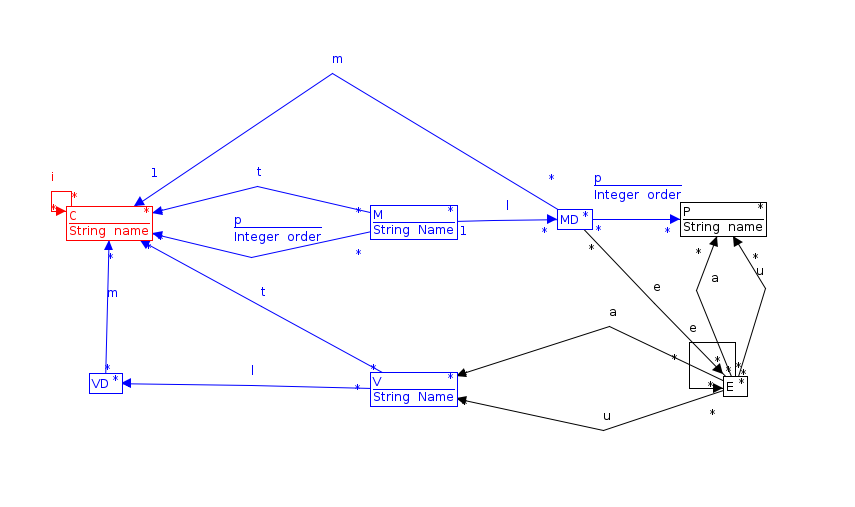
\includegraphics[width=\textwidth]{typeGraph.png}
  \end{myfig}

  La figure~\ref{typeGraph} est un exemple de graph de type, on peut observer toutes les relations possibles entre les noeuds typés et les arrêtes typées.

  Voici quelques exemples:
  \begin{itemize}[label=\textbullet]
    \item Un noeud de type C peut hériter d'un autre noeud de type C.
    \item Un noeud de type MD contiendra des noeuds de type E et appartiendra à un noeud de type C
    \item Un noeud de type V aura comme type un noeud de type C
    \item Un noeud de type E pourra mettre à jour ou bien accèder à un noeud de type V
  \end{itemize}


  \subsection{Les graphs de programme}

  Un graph de programme est un graph typé et labelé représentant la structure du code source d'un programme. Il est composé de noeuds typés reliés par des arrêtes typées. Ses noeuds et ses arrêtes prennent les valeurs vu dans le graph de type figure~\ref{typeGraph} et sont agrémentés d'un nom et/ou d'autres attributs. La figure~\ref{typedGraph} est un exemple de graph de programme.

  \subsubsection{Definition}
  \(G \) est composé d'un ensemble de noeuds labelés et d'arrêtes labelées, c'est un graph formé de triplet, ({$V_G$},{$E_G$},\(nlabg \)), ou {$V_G$} est un ensemble de noeuds, \(nlabg \) est une function de nomage de noeud et {$E_G$} est un ensemble d'arrêtes. Les arrêtes sont représentées par un triplet (noeud depart, label, noeud destination).

  Dans un graph de programme les entité (classes, variables, méthodes et paramètres) sont représentés par des noeuds dont le label est une paire composée d'un nom et d'un type. Et les relations entre ces différentes entités (héritage, appelle de méthodes, appartenance) sont représentées par des arrêtes.

  Ces arrêtes possèdent un label dans le but de faire la différence entre les arrêtes de même type ayant le même noeud source et le même noeud destination.

  \begin{myfig}{typedGraph}{Graph de programme}
    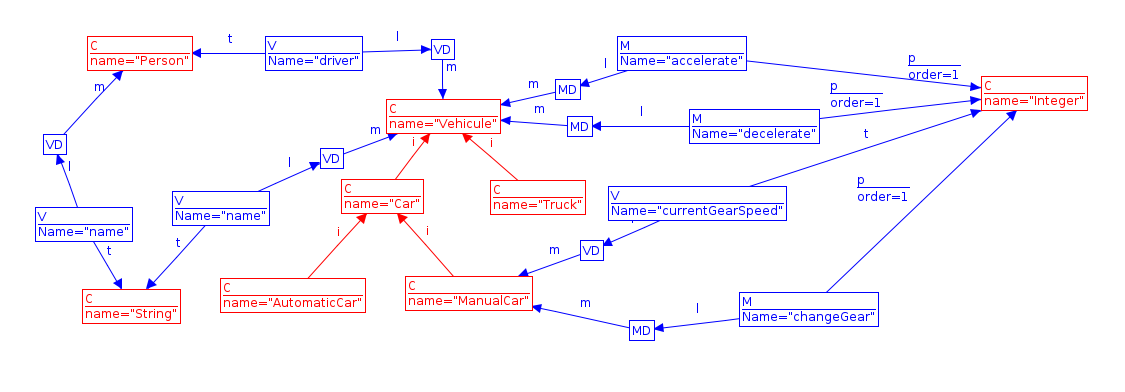
\includegraphics[width=\textwidth]{typedGraph.png}
  \end{myfig}

  \subsection{Les graph d'expression}

  Dans la section~\ref{subsec:graphExpression} nous avons évoqué les graphs d'expressions en vue de représenter des contraintes supplémentaires.

  Ces graphs possèdent des arrêtes dont les labels peuvent être des expressions régulières, ceci permet de représenter un ensemble de graph à partir d'un seul.

  Il suffit de remplacer les expressions régulières par leurs valeurs et de créer un graph pour chacune de celle çi. Exemple figure~\ref{graphExpression}

  \begin{myfig}{graphExpression}{Graph d'expression}
    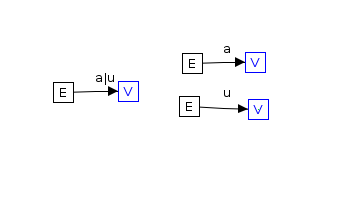
\includegraphics{graphExpression.png}
  \end{myfig}

  A gauche de la figure~\ref{graphExpression}, se trouve un graph avec une arrête dont le label est une expression régulières.
  A droite, sont représentés les deux graphs issu du premier graph, une expression méttant à jour une variable et une expression accédant à une variable.

  L'exemple reste assez simple mais vous pouvez imaginer un graph qui peut representer des centaines d'autres graphs.

  \section{Cas d'étude}

  Dans ce rapport, nous étudierons deux refactoring en particulier.

  \begin{enumerate}
    \item PullUpMethod qui consiste à supprimer une méthode présente dans une ou plusieur classes enfant et à l'insérer dans la classe parent.
    \item EncapsulateVariable qui consiste à imposer l'accès et la mise à jour d'une variable par l'intermédiaire de deux méthodes communément appelées getter et setter.
  \end{enumerate}

  Les exemples seront prit sur base du programme Transport, c'est un programme simple écrit en java permettant ces deux refactorings.

  Certains exemples seront donné sous forme de graph. Dans la plupart des cas, ces graphs ont été réalisé grâce à l'outil AGG.

  Les caractèristique de AGG sont:

  \begin{itemize}[label=\textbullet]
    \item Représenter des structures de donnée sous forme de graph qui peuvent être typé par un graph de type.
    \item Spécifier des règles sur un graph
    \item Spécifier des NAC pour exprimé la non-existance de certaines structures lors de transformation de graph
    \item Application de transformation de graph
    \item Application séquentiel de transformation de graph
  \end{itemize}

  AGG est assez facile à prendre en main, surtout grâce aux exemples fournis. Il m'a aidé à comprendre certains concepts comme les NACs et m'a été très utile durant toute la rédaction de ce rapport.

  \subsection{Programme Transport}

  \begin{lstlisting}[frame=single]
    public class Vehicule {
    public String name;
    public Person driver;

    public void accelerating(int amount) {

    }

    public void decelerate(int amount) {

    }
    }

    public class Truck extends Vehicule {

    }

    public class Person {
    public String name;
    }

    public class ManualCar {
    public int currentGearSpeed;

    public void changeGear(int number) {
    }
    }

    public class Car extends Vehicule {

    }

    public class AutomaticCar {

    }
  \end{lstlisting}

  \newpage
  \section{Refactoring}

  \subsection{Preservation du comportement}
  \label{subsec:preservationDuComportement}

  La conservation du comportement d'un programme est une chose primordiale lors d'un refactoring.
  Malheureusement , il n'est pas facile de définir en quoi consiste réellement cette préservation.

  Par ailleurs il sera nécessaire de trouver une définition suffisante garantissant que le programme effectuera les mêmes actions avant et après le refactoring.

  Dans cette optique, nous nous concentrerons ici sur trois proprietés.

  \begin{itemize}[label=\textbullet]
    \item Préservation de l'accès, chaque méthode accédera au moins à toutes les variables qu'elle accédait avant le refactoring
    \item Préservation de la mise à jour, chaque méthode mettera à jour au moins toutes les variables qu'elle mettait à jour avant le refactoring
    \item Préservation de l'appelle, chaque méthode appellera au moins toutes les méthodes qu'elle appelait avant le refactoring
  \end{itemize}

  \subsection{Transformation de graph}

  Pour représenter un refactoring appliqué sur le code source d'un programme, on applique des transformations de graph sur le graph de programme.

  Il reste cependant quelques problèmes:

  \begin{enumerate}
    \item Certains types de refactoring modifie une partie variable d'un programme, ce qui les rend impossible à représenter grâce à une simple transformation.
    Il faut donc appliquer plusieurs transformations l'une après l'autre dans un ordre spécifique, pour cela nous auront besoin d'un mecanisme de réecriture de graph controllé.

    \item La representation d'un refactoring devra être représenté sous forme générique et non spécifique aux noms des classes/méthodes contenues dans le programme sur lequel il est appliqué.
    Pour cela une technique de production de graph avec paramètre va être emloyée.

    \item Il est possible que certaines arrêtes ne pointent plus vers aucuns noeuds suite a l'application d'un refatoring.
    Par exemple, elles accedaient à une variable qui est maintenant uniquement accessible par des méthodes (getter ou setter).
    Ces arrêtes ne sont normalement pas autorisé mais les éviter serait beaucoup trop complexe.
    En effet les inclures dans les représentations de LHS et RHS créerait des ensembles LHS et RHS infinits.
    Pour pallier à ce problème on emploie un méchanisme appellé "embedding mechanism" qui autorise ces arrêtes oprhelines et qui présisera comment les rediriger vers un autre noeud.

  \end{enumerate}

  \subsubsection{Règles de transformation}

  Quelques notions doivent être définies avant de pouvoir appliquer une production à un graph:

  \begin{enumerate}
    \item \(G\) étant un graph, un sous graph de \(G\) contient un ensemble de noeuds de \(G\) et uniquement les arrêtes reliant les noeuds contenu dans ce sous graph.

    \item Lorsque l'on applique un mappage sur les noeuds de \(G\), on applique automatiquement un mappage sur les arrêtes reliant ces noeuds.

    \item \(G\) et \(K\) étant des graphs, une occurence de \(K\) dans \(G\) nécessite que toutes les arrêtes entre les noeuds correspondant existent.

  \end{enumerate}

  \tikzstyle{weight} = [font=\small]
  \tikzstyle{edge} = [draw,line width=2pt,-,black]
  \tikzstyle{vertex}=[circle,fill=black!25,minimum size=10pt,inner sep=0pt]
  \begin{myfig}{sousGraph1}{Graph}
    \begin{tikzpicture}[scale=1.8, auto,swap]

      % First we draw the vertices
      \foreach \pos/\name in {{(0,2)/b}, {(2,2)/c}, {(1,1)/e},
      {(0,0)/a}, {(2,0)/d}}
      \node[vertex] (\name) at \pos {$\name$};
      % Connect vertices with edges and draw weights
      \foreach \source/ \dest /\weight in {a/b/1, c/b/2,c/d/3,d/a/4,
      e/c/5, b/e/6}
      \path[edge] (\source) -- node[weight] {$\weight$} (\dest);

    \end{tikzpicture}
  \end{myfig}


  \begin{myfig}{sousGraph2}{Exemple sous graph valide / invalide}
    \tikzstyle{edge} = [draw,line width=2pt,-,green]
    \tikzstyle{vertex}=[circle,fill=green!25,minimum size=10pt,inner sep=0pt]
    \begin{tikzpicture}[scale=1.8, auto,swap]

      % First we draw the vertices
      \foreach \pos/\name in {{(0,2)/b}, {(2,2)/c}, {(1,1)/e}}
      \node[vertex] (\name) at \pos {$\name$};
      % Connect vertices with edges and draw weights
      \foreach \source/ \dest /\weight in {c/b/2,
      e/c/5, b/e/6}
      \path[edge] (\source) -- node[weight] {$\weight$} (\dest);

      \tikzstyle{edge} = [draw,line width=2pt,-,red]
      \tikzstyle{vertex}=[circle,fill=red!25,minimum size=10pt,inner sep=0pt]

      % First we draw the vertices
      \foreach \pos/\name in {{(3,2)/b}, {(5,2)/c}, {(4,1)/e}}
      \node[vertex] (\name) at \pos {$\name$};
      % Connect vertices with edges and draw weights
      \foreach \source/ \dest /\weight in {c/b/2, b/e/6}
      \path[edge] (\source) -- node[weight] {$\weight$} (\dest);
    \end{tikzpicture}
  \end{myfig}

  \subsubsection{Definition}

  La définition mathématique est donnée dans l'article~\cite[p.~15]{mainArticle}.

  Je vais tout de même l'expliquer à l'aide des figures~\ref{sousGraph1} et \ref{sousGraph2}.

  \(G\) et \(H\) sont des graphs, \(m\) est une fonction de mappage de \(L\) vers \(G\) et \(n\) est une fonction de mappage de \(R\)  vers \(H\) .

  \(m(v)\) est un sous graph de \(G\) et \(n(w)\) est un sous graph de H.

  {$V_H$} est égale au graph \({$V_G$} \setminus~m({$V_L$})~\cup~n({$V_R$})\). De facon très imagée on peut voir ça comme un oeuf dont on retirerai le jaune d'oeuf et on le remplacerait par un autre.

  $\underset{in}{Emb}$ est utilisée pour rediriger les arrêtes partant de noeuds contenu dans \( {$V_G$}~\setminus~m({$V_L$}) \) qui pointais vers des noeuds contenu dans \( m({$V_L$}) \) à des arrêtes d'un noeuds de \( {$V_H$} \setminus n({$V_R$}) \) à un noeuds de \( n({$V_R$}) \).

  $\underset{out}{Emb}$ est utilisée pour rediriger les arrêtes partant de noeuds contenu dans \( m({$V_L$}) \) qui pointais vers des noeuds de \( {$V_G$}~\setminus~m({$V_L$}) \) à des noeuds de \(n({$V_R$}) \) vers des neouds de \( {$V_H$}~\setminus~n({$V_R$}) \).

  \begin{myfig}{sousGraph}{$\underset{out}{Emb} ~ et ~ $\underset{out}{Emb}}
    \tikzset{>=latex}
    \begin{tikzpicture}
      \node[] at (1,5) {L};
      \draw (2,4) ellipse (1cm and 0.5cm);
      \node[] at (2,4) {V};

      \draw[->] (5,4) -- +(1,0);
      \draw[->] (2,3) -- +(0,-1) node[anchor=south] {m};

      \node[] at (8,5) {R};
      \draw (9,4) ellipse (1cm and 0.5cm);
      \node[] at (9,4) {W};

      \draw[->] (9,3) -- +(0,-1) node[anchor=south] {n};

      \node[] at (0,1) {G};
      \draw (2,0) ellipse (2cm and 1cm);
      \draw (2,0) ellipse (1cm and 0.5cm);
      \node[] at (2,0) {m(v)};

      \draw[->] (5,0) -- +(1,0);

      \draw (3.5,0) node[anchor=south] (e) {\textbullet};
      \draw (2.5,0) node[anchor=south] (f) {\textbullet};

      \draw (0.5,0) node[anchor=south] (g) {\textbullet};
      \draw (1.5,0) node[anchor=south] (h) {\textbullet};

      \draw[-latex] (e.west) to[out=90,in=70] (f.east);

      \draw[-latex] (h.west) to[out=70,in=90] (g.east);

      \node[] at (7,1) {H};
      \draw (9,0) ellipse (2cm and 1cm);
      \draw (9,0) ellipse (1cm and 0.5cm);
      \node[] at (9,0) {n(w)};

      \draw (10.5,0) node[anchor=south] (a) {\textbullet};
      \draw (9.5,0) node[anchor=south] (b) {\textbullet};

      \draw (7.5,0) node[anchor=south] (c) {\textbullet};
      \draw (8.5,0) node[anchor=south] (d) {\textbullet};

      \draw[-latex] (a.west) to[out=90,in=70] (b.east);

      \draw[-latex] (d.west) to[out=70,in=90] (c.east);

    \end{tikzpicture}

  \end{myfig}


  \begin{myfig}{LHSRHSPullUpMethod}{LHS et RHS}
    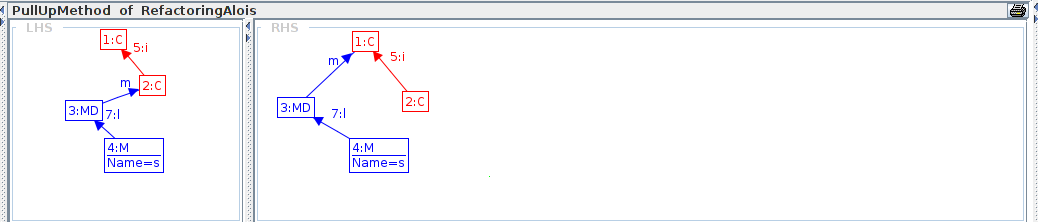
\includegraphics[width=\textwidth]{LHSRHSPullUpMethod.png}
  \end{myfig}

  \subsection{Précondition de refactoring}
  Les préconditions servent à définir un sous graph ou un ensemble de sous graph ne pouvant pas être présent avant d'appliquer le refactoring.
  Nous pourrions également employé des postconditions pour interdire certains sous graphs dans le graph résultat
  mais les préconditions sont plus adaptée car on évite d'appliquer des transformations sur un graphs et ensuite seulement de détecter les erreurs.

  \begin{myfig}{NACPullUpMethod}{NAC}
    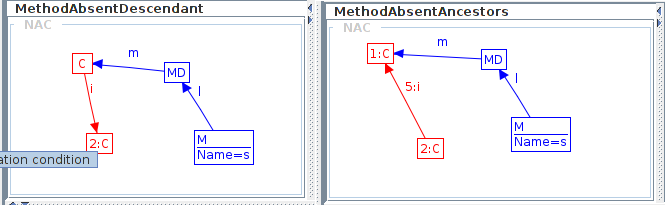
\includegraphics[width=\textwidth]{NACPullUpMethod.png}
  \end{myfig}

  La figure~\ref{NACPullUpMethod}, représente les deux préconditions nécessaire pour pouvoir appliquer le refactoring PullUpMethod.
  Elle spécifie que aucuns ancêtres ni descendants de la classe ne peut posséder cette méthode avant le refactoring.


  \section{Application sur le programme transport}

  \subsection{Encapsulate Variable}

  Encapsuler une variable dans une classe est une opération souvent éffectué par les programmeurs.
  Elle consiste à rendre une variable public, privée et à ajouter un accesseur public et un setter public pour continuer à accéder ou à mettre à jour cette variable.

  Lors d'un refactoring cela consiste à changer la visibilité de la variable et à créer deux nouvelles methodes. Ensuite il faut changer tout les accès ou/et mise à jour de la variable par des appels au deux méthodes crées.

  \subsubsection{Conditions}

  \begin{itemize}[label=\textbullet]
    \item Les deux nouvelles méthodes crées ne sont pas déjà présente dans la classe
    \item Les deux nouvelles méthodes crées ne sont pas déjà présente dans ses ancêtres
    \item Les deux nouvelles méthodes crées ne sont pas déjà présente dans ses descendants.
  \end{itemize}

  \subsubsection{Contraintes}

  \begin{enumerate}
    \item est préservée car on ne crée ni ne bougeons aucune variable.
    \item est préservée car la condition stipules qu'ils ne faut pas que des méthodes comportant les même définition que le getter ou le setter soient présente.
    \item est préservée car on crée deux méthodes accédant une variable dans la même classe.
    \item est préservée car le paramètre de la méthodes setter est employée uniquement dans la définition de cette méthode.
  \end{enumerate}

  \subsubsection{Avant}

  \begin{lstlisting}[frame=single]
    public class Person {
    public String name;
    }
  \end{lstlisting}

  \subsubsection{Après}

  \begin{lstlisting}[frame=single]
    public class Person {
    private String name;

    public String GetName(){
    return name;
    }

    public void SetName(String n){
    name=n;
    }
    }
  \end{lstlisting}

  \subsubsection{Représentation graphique}

  \begin{myfig}{beforeEncapsulateVariable}{Before Encapsulate Variable}
    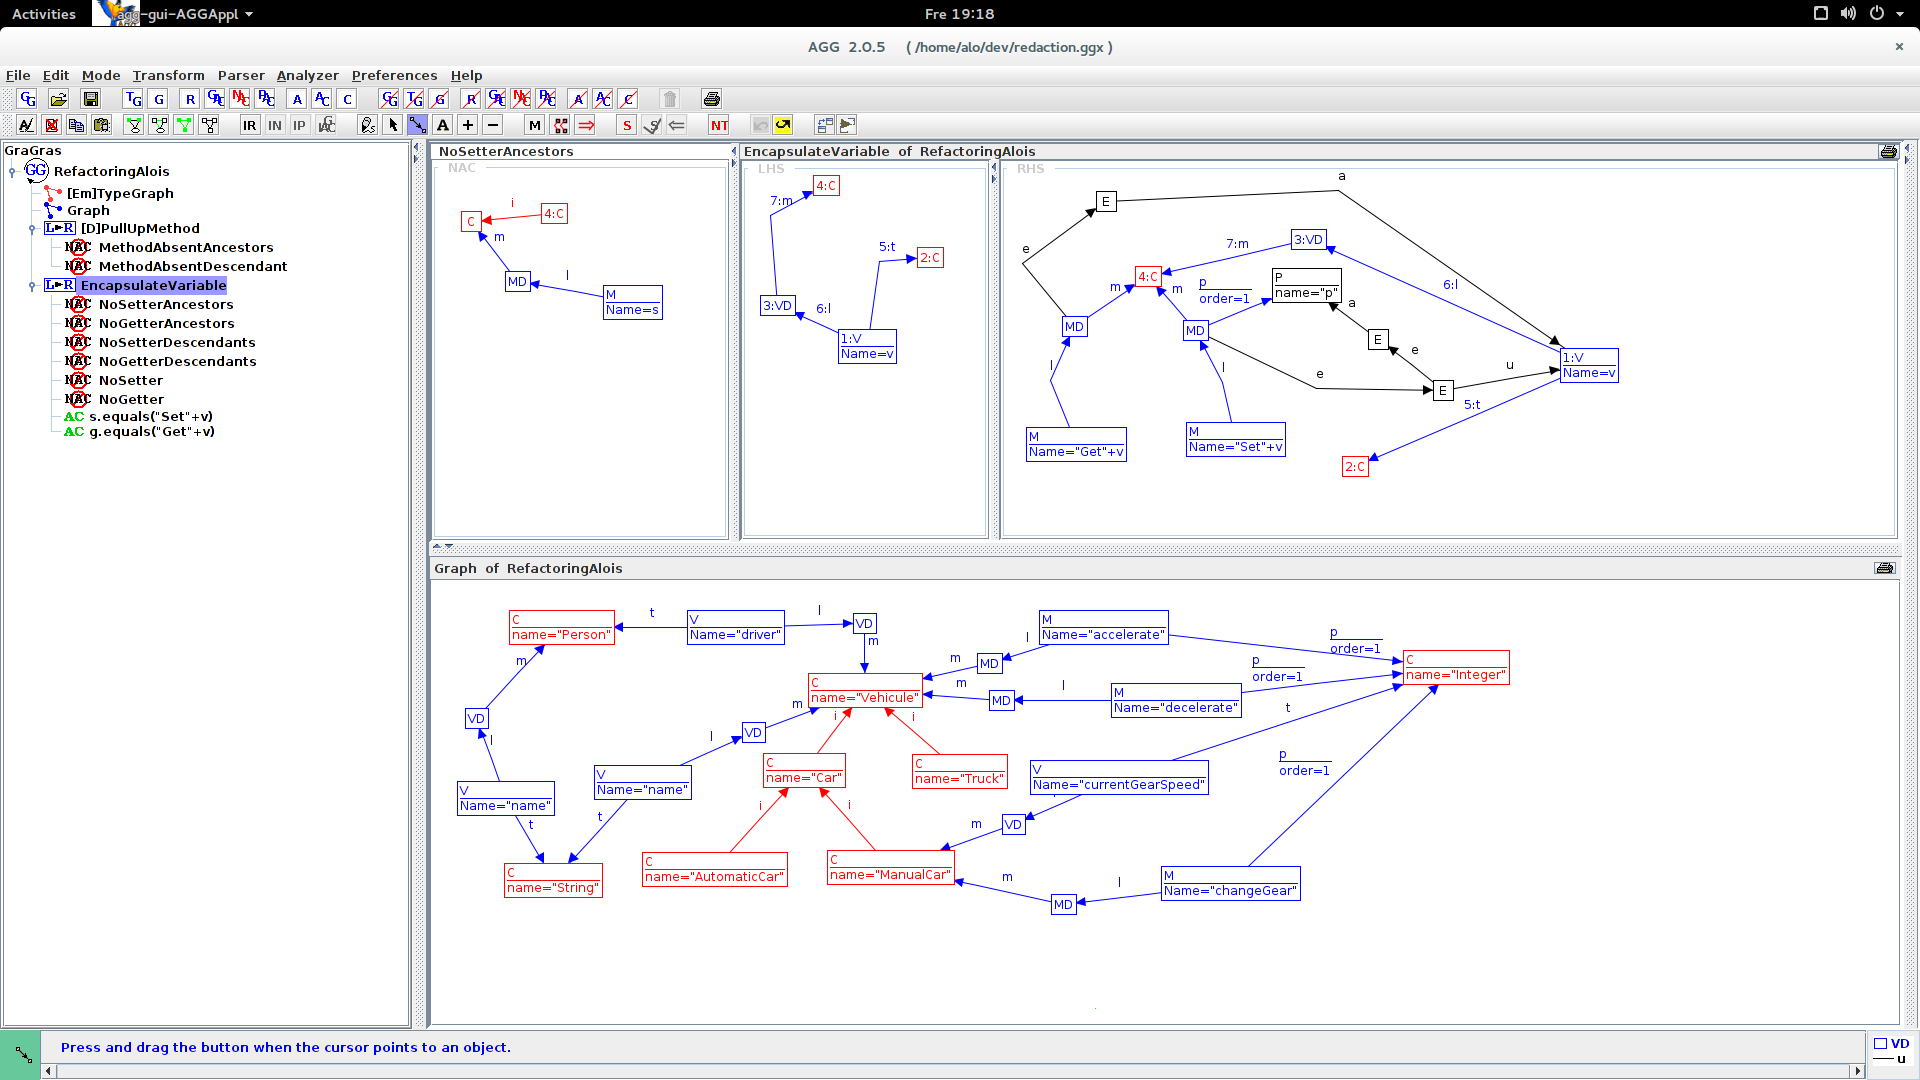
\includegraphics[width=\textwidth]{beforeEncapsulateVariable.png}
  \end{myfig}

  Dans le haut de la figure~\ref{beforeEncapsulateVariable} se trouve la LHS qui représente le sous graph du programme à transformer.
  A droite, nous avons RHS qui représente la structure de ce sous graph après la transformation.
  Et en dessous nous avons le graphique du programme.

  \begin{myfig}{afterEncapsulateVariable}{After Encapsulate Variable}
    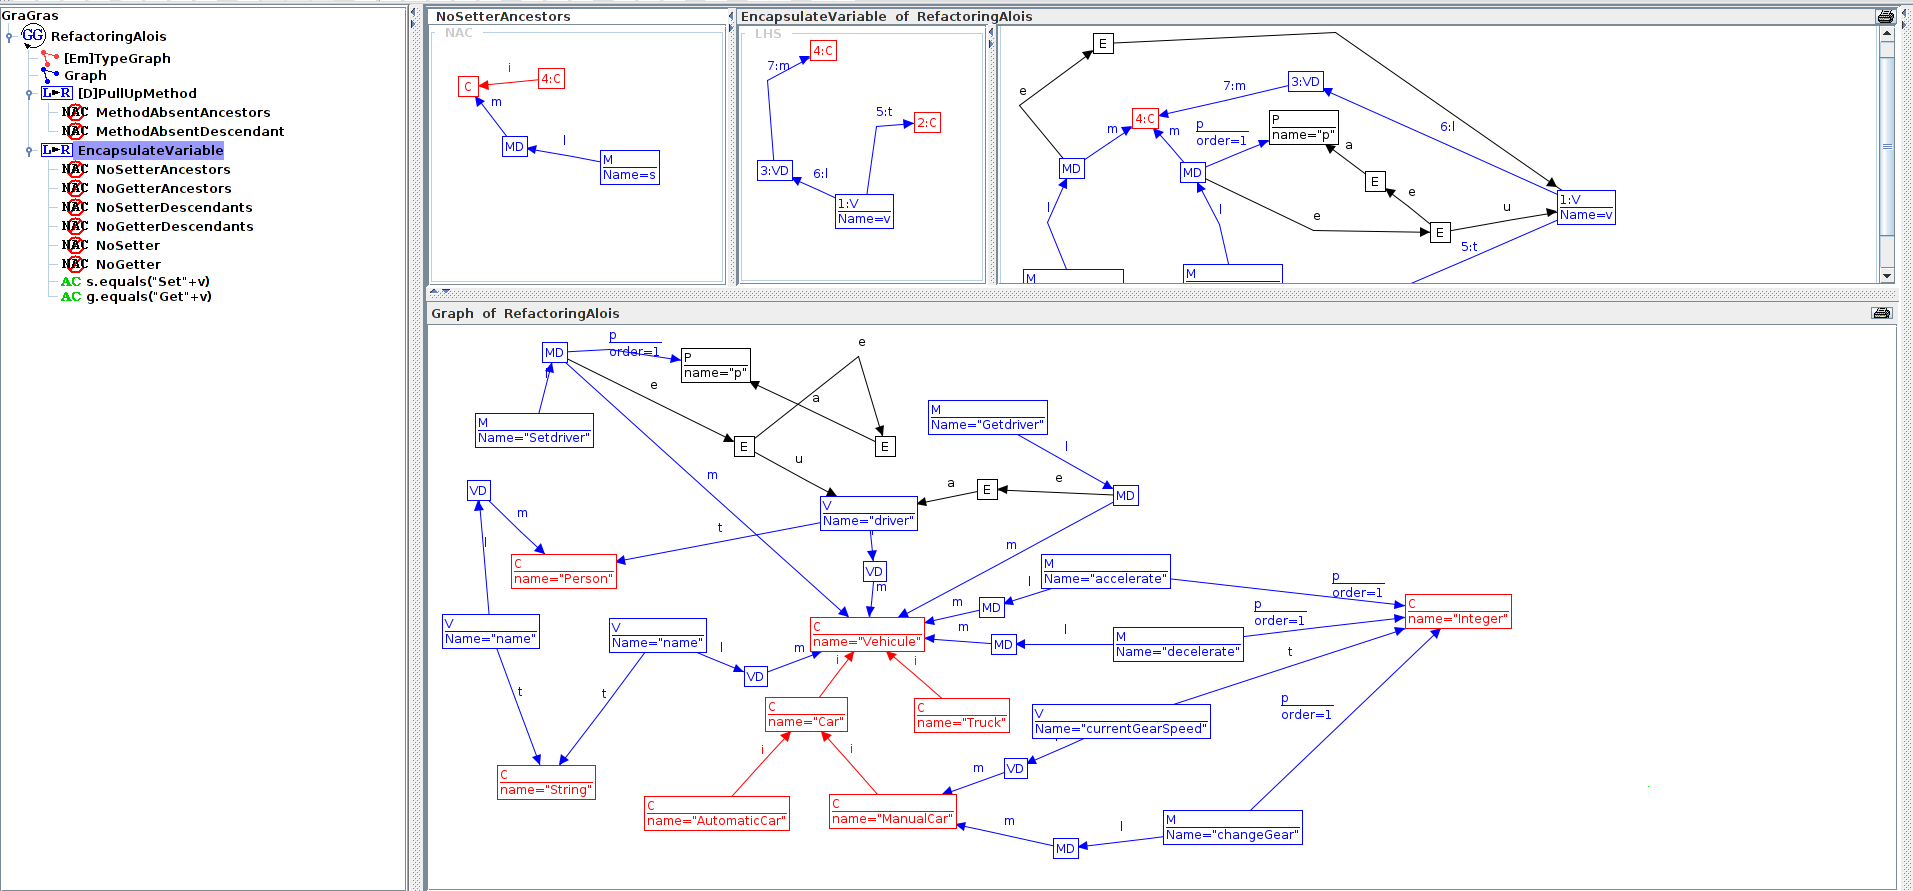
\includegraphics[width=\textwidth]{afterEncapsulateVariable.png}
  \end{myfig}

  Ici dans la figure~\ref{afterEncapsulateVariable} nous avons les mêmes éléments au dessus mais la partie inférieur à changer.
  Elle représente le graphique après l'application de la/les transformations. On peut voir que de nouveaux noeuds et de nouvelles arrêtes ont été créer pour représenter les deux nouvelles méthodes.

  Je n'ai laissé que la transformation du sous graph lié à la variable "driver" pour une meilleure visibilité.

  \subsection{Pull Up Method}

  Cela consiste à déplacer une méthode présente dans une ou plusieur classes enfant dans leur classe parent.

  \subsubsection{Conditions}

  \begin{itemize}[label=\textbullet]
    \item La classe parent ne peut pas déjà contenir une méthode ayant la même signature
    \item Aucune des variables directement accédée ou modifiée par la méthode ne peut être en dehors de la portée (scope) de la classe parent.
  \end{itemize}

  \subsubsection{Contraintes}

  \begin{enumerate}
    \item est préservée car on ne crée ni ne bougeons aucune variable.
    \item est préservée grâce à la précondition qui stipule qu'il ne peut pas se trouver une méthode avec la même signature dans la classe parent.
    \item est préservée grâce à la précondition qui stipule que la définition de la méthode bougée ne doit pas accéder à des variables en dehors du scope du parent.
    \item est préservée car on ne crée ni ne modifie aucune méthode.
  \end{enumerate}

  \subsubsection{Avant}
  \begin{lstlisting}[frame=single]
    public class Vehicule {
    public String name;
    public Person driver;

    public void accelerating(int amount) {
    }

    public void decelerate(int amount) {
    }
    }

    public class Car extends Vehicule {

    }

    public class ManualCar extends Car {
    public void changeGear(int speed){
    }
    }
  \end{lstlisting}

  \subsubsection{Après}
  \begin{lstlisting}[frame=single]
    public class Vehicule {
    public String name;
    public Person driver;

    public void accelerating(int amount) {

    }
    public void decelerate(int amount) {
    }

    public void changeGear(int speed){
    }
    }

    public class Car extends Vehicule {

    }

    public class ManualCar extends Car {

    }
  \end{lstlisting}

  \subsubsection{Représentation graphique}

  \begin{myfig}{beforePullUpMethode}{Before PullUp Methode}
    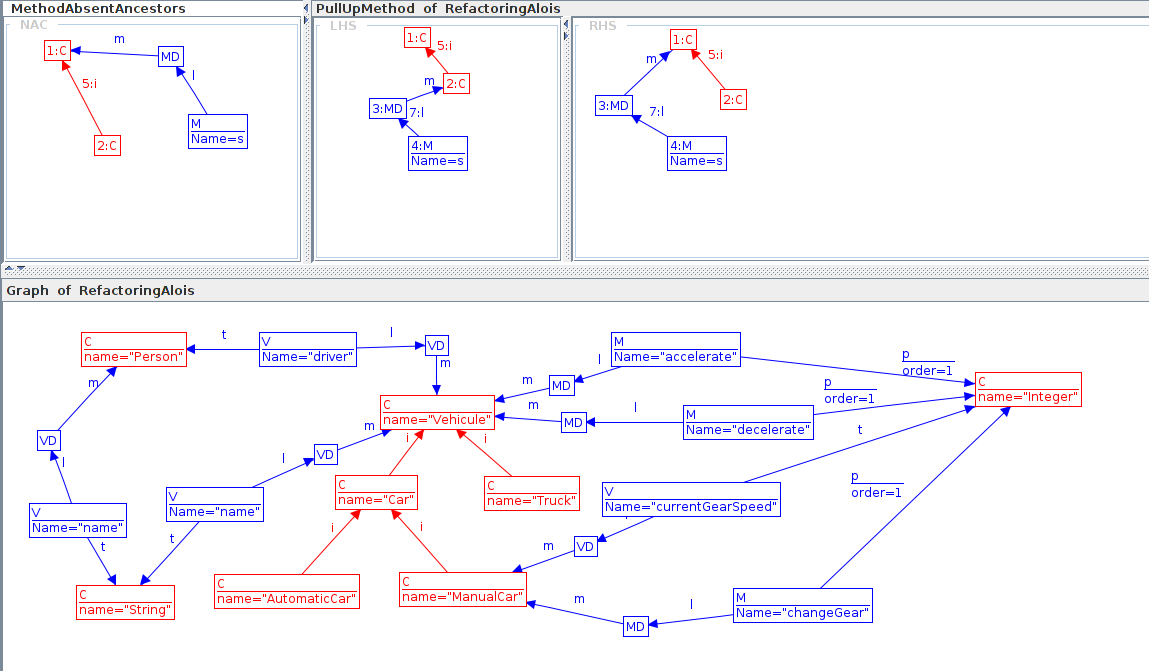
\includegraphics[width=\textwidth]{beforePullUpMethode.png}
  \end{myfig}

  En haut à gauche de la figure~\ref{beforePullUpMethode} se trouve la LHS qui représente la structure du sous graph à transformer.
  En haut à droite de la figure~\ref{beforePullUpMethode} se trouve la RHS qui représente la structure de ce sous graph après la transformation.
  En dessous nous avons le graphique du programme.

  \begin{myfig}{afterPullUpMethod}{After PullUp Methode}
    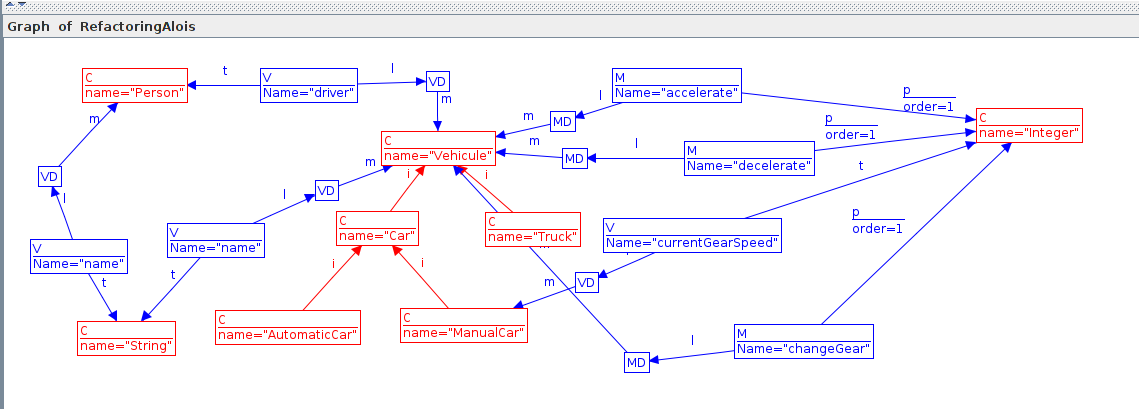
\includegraphics[width=\textwidth]{afterPullUpMethod.png}
  \end{myfig}

  Dans la figure~\ref{afterPullUpMethod} la partie du dessous à changé et représente le programme après avoir appliqué la transformation.
  Après avoir remonté la méthode de la classe ManualCar dans la classe Vehicule,
  on peut observer que le lien de la méthode "changeGear" vers la classe ManualCar n'existe plus. Et qu'un nouveau lien a été créé vers la classe Vehicule.

  \section{Préservation du comportement du programme}

  Jusqu'ici nous avons définit des mécanismes permettant de refactorer un programme à l'aide de graph.Il nous reste encore à prouver que ce programme conserve son comportement à la suite de ces transformations.

  Le but de cette partie est de démontrer que certaines propriétés du programme sont preservée après un refactoring:
  \begin{itemize}[label=\textbullet]
    \item l'accès aux variables
    \item la mise à jour de variable
    \item l'appelle de méthode
  \end{itemize}

  Pour cela nous avons besoin d'introduire le concept d'une fonction de tracking appelée, \(tr\).

  \subsection{Définition, Préservation d'une expression de graph}

  \(GE\) étant un graph d'expression, \(G\) et \(H\) étant des graphs de programme. La fonction \(tr: {$V_G$} \rightarrow {$V_H$}\) est un mappage de noeud tels que pour chaque occurence \( oc \) de GE dans G, La composition de fonction  \(tr \circ oc \) est une occurence de GE dans H.

  Pour chaque production de graph une fonction tr existe et mappe les noeuds de LHS dans ceux de RHS.

  \subsection{Définition, Fonction de tracking}
  Si \(G\) derive \(H\) grâce à une production \( P = (L,R,$\underset{in}{Emb}$ ,$\underset{out}{Emb}$ ) \) via m et n, alors la fonction de tracking tr : \( {$V_G$} \rightarrow {$V_H$} \) est définie comme suit :

  tr(v) = { \(n \circ trp \circ m-1(v)\) , si v est une node de \(m(L)\) \\ v, si v n'est pas une node de \(m(L)\)

  \[tr(v) = \left\{
  \begin{array}{lr}
    \( n \circ trp \circ m^{-1}(v) \) : si v est une node de m(L)\\
    \(v \) : si v n'est pas une node de m(L)
  \end{array}
  \right.
  \]

  Cette définition mathématique définit :
  \begin{itemize}[label=\textbullet]
    \item Pour tout noeud contenu dans \( {$V_L$} \) , la fonction \(m^{-1}(v)\) va chercher le noeud dans {$V_G$} et le mappe dans \( L \) ensuite la fonction de tracking mappe le noeud de  \( L \)
    dans  \( R \)  et enfin la fonction \( n \) mappe le noeud de  \( R \)  dans {$V_H$}.
    \item Pour tout les autres noeuds, ils ne faut rien faire.
  \end{itemize}

  \subsection{Préservation du comportement : Encapsulate Variable}

  \subsubsection{Production et table de correspondance}

  \begin{myfig}{embedding}{méchanisme "embedding"}
    \begin{center}
      \begin{tikzpicture}[->,>=stealth',shorten >=1pt,auto,node distance=3cm,
        thick, label distance=-1mm, label position=45, every label/.style={red}]


        \node at (0,2) [draw,thick,minimum width=1cm,minimum height=0.5cm,label=2] (typeG) {C};
        \node [draw,thick,minimum width=1cm,minimum height=0.5cm,label=1] at (0,0)  (varLeft) {var V};

        \draw[red, arrows={-Triangle[angle=90:10pt,red,fill=black]}]  (1,1) -- (3,1);
        \node[red] at (2,0.5) {P1};

        \node (rect) at (4,2) [draw,thick,minimum width=1cm,minimum height=0.5cm,label=3] (setter) {Setter M};
        \node at (4,4) [draw,thick,minimum width=0.5cm,minimum height=0.5cm] (p) {P};
        \node (rect) at (4,0) [draw,thick,minimum width=1cm,minimum height=0.5cm,label=4] (getter) {Getter M};
        \node at (6,2) [draw,thick,minimum width=1cm,minimum height=0.5cm,label=2] (typeD) {C};
        \node (rect) at (6,0) [draw,thick,minimum width=1cm,minimum height=0.5cm,label=1] (varRight) {var V};

        \path[every node/.style={font=\sffamily\small}]
        (varRight) edge node {t} (typeD)
        (getter) edge node [right] {t} (typeD)
        (p) edge node {t} (typeD)
        (varLeft) edge node {t} (typeG)
        (setter) edge [left] node [right] {1.p} (p)

      \end{tikzpicture}
    \end{center}

    \begin{center}
      \begin{tikzpicture}[->,>=stealth',shorten >=1pt,auto,node distance=3cm,
        thick, label distance=-1mm, label position=45, every label/.style={red}]
        \tikzstyle{EdgeStyle}=[bend left]

        \node at (0,2) ["180:$2$", draw,thick, minimum width=1cm, minimum height=0.5cm] (setter) {Setter M};
        \node at (0,0) [draw,thick,minimum width=1cm,minimum height=0.5cm,label=3] (getter) {Getter M};
        \node at (3,2) [draw,thick,minimum width=1cm,minimum height=0.5cm,label=1] (varLeft) {var V};
        \node (rect) at (3,0) [draw,thick,minimum width=1cm,minimum height=0.5cm] (vdLeft) {VD};
        \node (rect) at (3,-2) [draw,thick,minimum width=1cm,minimum height=0.5cm] (class) {C};

        \node at (1,1) [draw,thick,minimum width=0.5cm,minimum height=0.5cm] (eU) {E};
        \node at (-1,1) [draw,thick,minimum width=0.5cm,minimum height=0.5cm] (mdU) {MD};
        \node at (1,-1) [draw,thick,minimum width=0.5cm,minimum height=0.5cm] (eA) {E};
        \node at (-1,-1) [draw,thick,minimum width=0.5cm,minimum height=0.5cm] (mdA) {MD};

        \draw [red, arrows={-Triangle[angle=90:10pt,red,fill=black]}]  (4,1) -- (6,1);
        \node[red] at (5,0.5) {P2};

        \node at (7,2) [draw,thick,minimum width=1cm,minimum height=0.5cm,label=4] (mdSetter) {MD};
        \node at (7,0) [draw,thick,minimum width=1cm,minimum height=0.5cm,label=2] (setter) {Setter M};
        \node at (9.5,2) [draw,thick,minimum width=1cm,minimum height=0.5cm,label=1] (varRight) {var V};
        \node at (9.5,0) [draw,thick,minimum width=1cm,minimum height=0.5cm,label=0] (vdRight) {VD};
        \node at (12,2) [draw,thick,minimum width=1cm,minimum height=0.5cm,label=5] (mdGetter) {MD};
        \node at (12,0) [draw,thick,minimum width=1cm,minimum height=0.5cm,label=3] (getter) {Getter M};

        \path[every node/.style={font=\sffamily\small}]
        (setter) edge [left] node [right] {l} (mdSetter)
        (getter) edge [left] node [right] {l} (mdGetter)
        (mdGetter) edge node {a} (varRight)
        (mdSetter) edge node {u} (varRight)
        (eU) edge [left] node {u} (varLeft)
        (eA) edge node  {a} (varLeft)
        (varLeft) edge [left] node [right] {l} (vdLeft)
        (varRight) edge [left] node [right] {l} (vdRight)
        (vdLeft) edge [left] node [right] {m} (class)
        (mdA) edge node {e} (eA)
        (mdU) edge node {e} (eU)
      \end{tikzpicture}
    \end{center}


    \begin{tabular}{ | l | l |  l |}
      \hline production & arrêtes entrantes & arrêtes sortantes  \\ \hline
      P1 : & (\(a,1) {\rightarrow} (a,1)\) &  (\(t,1) {\rightarrow}(t,1),(1.p,2),(t,3)\)   \\ \hline
      & (\(u,1) {\rightarrow} (u,1)\) & (\ (l,1) {\rightarrow} (l,1)\)  \\ \hline
      P2 : & (\(a,1) {\rightarrow} (c,3)\) &  (\(m,0) {\rightarrow} (\(m,0),(m,4),(m,5)\)\)    \\ \hline
      & (\(u,1) {\rightarrow} (c,2)\) &  (\(t,1) {\rightarrow} (t,1)\)  \\ \hline
    \end{tabular}
  \end{myfig}

  Sur la firgure~\ref{embedding} on peut observer différentes chose grâce aux graphs mais égalemment à la table :

  \begin{itemize}[label=\textbullet]
    \item Les noeuds ayant les mêmes numéros sont des noeuds conservés entre les productions.
    \item Le type de la variable reste inchangé
    \item Le type de retour du getter est identique à celui de la variable
    \item Le type du paramètre du setter est identique à celui de la variable
    \item Les arrêtes de types \(a\) ou \(u\) sont changées en arrêtes de types \(c\) pointant vers le getter et le setter.
    \item Les nouvelles définitions de méthodes appartienne à la même classe que la définition de variable
  \end{itemize}

  Afin de montrer que notre approche est correcte, je vais prouver la préservation de l'accès à une variable lors d'un refactoring Encapsulate Variable.
  Le graph d'expression  \(MD \underset{( e ) * a}{\rightarrow} V \underset{t}{\rightarrow}  VD\) représente toutes les possibilités d'accès possible à une variable depuis une définition de méthode.

  Garantir la préservation de l'accès consite à prouver que pour chaque occurance de \(MD \underset{( e ) * a}{\rightarrow} V \underset{t}{\rightarrow} VD\) dans le graph initial, il y a une occurence correspondante dans le graph resultat.

  Pour cela je vais prouver que les productions P1 et P2 préserve les propriétés \(GE1 = MD \underset{( e ) * a}{\rightarrow} V \) et  \(GE2 = V \underset{t}{\rightarrow}  VD\).

  \begin{enumerate}
    \item

    \begin{itemize}[label=\textbullet]

      Pour la production P1. $G$ et $H$ étant des graphs et $G$ derivant $H$ en fonction de $P1$ via $m$ et $n$, et tr étant la fonction de tracking. oc :  \( {V_{GE1}} {\rightarrow} {V_G} \) est une occurence de  {$GE_1$} dans $G$.
      Alors il existe un chemin \( v_0 \underset{e}{\rightarrow} v_1 \underset{e}{\rightarrow} ... \underset{e}{\rightarrow} v_{n-1} \underset{a}{\rightarrow} v_n \) dans $G$
      ou {$v_0$} est la node 1 de {$V_{GE1}$} et {$v_n$} est la node 2 de $V_{GE1}$
      alors il doit exister un chemin \( tr(v_0) \underset{e}{\rightarrow} tr(v_1) \underset{e}{\rightarrow} ... \underset{e}{\rightarrow} tr(v_{n-1}) \underset{a}{\rightarrow} {v_n} \) dans $H$.

      \item Premièrement considérons les noeuds $tr(v_1) \underset{e}{\rightarrow} tr(v_2) \underset{e}{\rightarrow} ... \underset{e}{\rightarrow} tr(v_{n-1})$,
      il sont tous de type E et ne sont donc pas contenu dans la partie remplacée $m(L)$ de $G$.
      Les noeuds sont remappé tel quel dans $H$ et il existe donc un chemin $tr(v_1) \underset{e}{\rightarrow} tr(v_2) \underset{e}{\rightarrow} ... \underset{e}{\rightarrow} tr(v_{n-1})$ dans $H$.

      \item Deuxiemement pour le noeud {$v_0$} de type MD n'est pas contenu dans $m(L)$, $tr(v_0) = v_0 et donc tr(v_0) \underset{e}{\rightarrow} tr(v_1)$ est conservé dans $H$.

      \item Finalement pour le noeud {$v_n$} si il n'est pas contenu dans $m(L)$, $tr(v_n)= v_n et donc tr(v_{n-1}) \underset{a}{\rightarrow} tr(v_n)$ est conservé dans $H$.
      Si par contre $v_n$ est contenu dans $m(L)$ alors $v_n$ correspond au noeud 1 dans L et $tr(v_n)$ au noeud 1 dans la RHS de P1.
      Vu que ((a,1),(a,1)) \in $Emb_in$, $tr(v_{n-1}) \underset{e * a}{\rightarrow} tr(v_n)$ est conservé dans $H$.
      Vu que ((l,1),(l,1)) \in $Emb_out$ la variable garde sa définition de méthode.
      Vu que ((t,1),(t,1)) et ((t,1),(1.p,2)) et ((t,1),(t,3)) \in $Emb_out$ on peut garantir que la variable garde le même type, que le getter retourne le type de la variable et que le paramêtre du setter est bien
      du même que la variable.

      \item On peut deduire que GE1 est preservée par P1
    \end{itemize}

    \item

    \begin{itemize}[label=\textbullet]
      Pour la production P2. $G$ et $H$ étant des graphs et $G$ derive $H$ en fonction de $P2$ via $m$ et $n$, et $tr$ est la fonction de tracking.
      oc :  \( {$V_{GE1}$} {\rightarrow} {$V_G$} \) est une occurence de {$GE_1$} dans $G$.
      Alors il existe ue chemin \( {$v_0$} \underset{e}{\rightarrow} {$v_1$} \underset{e}{\rightarrow} ... \underset{e}{\rightarrow} v_{n-1} \underset{a}{\rightarrow} {$v_n$} \) dans $G$
      ou {$v_0$} est la node 1 de {$V_GE1$} et {$v_n$} est la node 2 de {$V_{GE1}$}
      alors il doit exister un chemin \( {$v_0$} \underset{e}{\rightarrow} {$v_1$} \underset{e}{\rightarrow} ... \underset{e}{\rightarrow} v_{n-1} \underset{a}{\rightarrow} {$v_n$} \) dans $H$.

      \item Premièrement considérons les noeuds $tr(v_1) \underset{e}{\rightarrow} tr(v_2) \underset{e}{\rightarrow} ... \underset{e}{\rightarrow} tr(v_n-1)$, il sont  tous de type E et ne sont donc pas contenu dans la partie remplacée $m(L)$ de $G$.
      Les noeuds sont remappé tel quel dans $H$ et il existe donc un chemin $tr(v_1) \underset{e}{\rightarrow} tr(v_2) \underset{e}{\rightarrow} ... \underset{e}{\rightarrow} tr(v_n-1)$ dans $H$.

      \item Deuxiemement pour le noeud {$v_0$} de type MD n'est pas pas contenu dans $m(L)$, tr({$v_0$}) = {$v_0$} et donc tr({$v_0$}) \underset{e}{\rightarrow} tr({$v_1$}) est conservé dans $H$.

      \item  Finalement pour le noeud {$v_n$} si il n'est pas contenu dans $m(L)$, tr{$v_n$})= {$v_n$} et donc $tr(v_{n-1}) \underset{a}{\rightarrow} tr(v_n)$ est conservé dans $H$.
      Si par contre {$v_n$} est contenu dans $m(L)$ alors {$v_n$} correspond au noeud 1 dans L et tr($v_n$) au noeud 1 dans la RHS de P1.
      Vu que ((a,1),(c,3)) \in $Emb_in$, $tr(v_{n-1}) \underset{e * a}{\rightarrow} tr(v_n)$ est conservé dans $H$ car l'expression appelera le getter qui lui mettera à jour la méthode.
      Vu que ((m,0),(m,4)) et ((m,0),(m,5)) \in $Emb_out$ on peut garantir que les méthodes seront accessible par $v_{n-1}$ car elle appartiennent à la même classe que la variable $v_n$.

      \item On peut deduire que GE1 est preservée par P2
    \end{itemize}

  \end{enumerate}

  \section{Conclusion}

  Le but de cet article était de prouver que le refactoring n'altérait pas le comportement d'un programme.
  A cet effet, il fallait créer un modèle simple et compatible avec les outils de refactoring actuels. Nous avons donc choisit de représenter le code source des programmes sous forme de graph
  et les transformations effectuées sur ce code source lors d'un refactoring sous forme de transformations de graph. Puis nous avons ajouté des contraintes à ces graphs de programme à l'aide d'un graph de type et d'autre mécanisme.

  Finalement il nous a fallu prouver la conservation de certaines propriétés dans ces graphs après les transformations.

  Malgré cela certains problèmes ont persister et nous ont amené à faire des ajouts et des compromis sur ce modèle:

  \begin{itemize}[label=\textbullet]
    \item Concernant les Préconditions, certaines contraintes on été mis de coté. Par exemple pour le refactoring PullUpMethod, on ne contronlle pas que le corps de la méthode soit identique mais uniquement la signature de la méthode.

    \item Concernant la représentation en graph, dans le but de supporté un large éventaille de language nous avons ajouté la possibilité d'attaché des attribus supplémentaires aux noeuds.

    \item Concernant le graph de type, toutes les contraites n'étaient pas représentable à l'aide de ce graph de type, nous avons donc introduit les graphs d'expressions.

    \item Concernant les transformations de graph, tout les types de refatoring ne pouvant pas être représenté à l'aide d'une seule transformation, nous avons permis de diviser un refactoring en une sucession de plusieurs transformations

    \item Concernant la préservation du comportement, Un concept de fonction de traquing a été employé pour permettre de traquer un noeud avant et après une transformation.
  \end{itemize}

  Il est difficile à dire si cette approche formelle peut réellement servir dans une approche pratique et être utilisée par un outil de refactoring.
  De plus bien que ce modèle soit relativement simple,il nécessite une bonne connaissance des graphs mathématiques.

  Toutefois, l'approche utilisée reste éfficace pour définir l'effet de chaque refactoring sur le code source d'un programme et son coté visuel si employé avec un outil comme AGG~\cite{aggSite} est un plus pour la compréhension.

  \newpage

  \begin{thebibliography}{9}

    \bibitem{aggManual}
    agg-team,
    The Agg 1.4.0 Development Environment The User Manual.

    \bibitem{mainArticle}
    Tom Mens, Niels Van Eetvelde, Serge Demeyer and Dirk Janssens,
    Formalizing Refactorings with Graph Transformations.

    \bibitem{secondArticle}
    Tom Mens and Tom Tourwe ,
    A Survey of Software Refactoring.

    \bibitem{otherArticle}
    Tom Mens, Gabriele Taentzer and Olga Runge,
    Detecting Structural Refactoring Conflicts Using Critical Pair Analysis.

    \bibitem{redaAcricle}
    Hadrien Mélot,
    Eléments de rédaction scientifique en informatique.

    \bibitem{aggHelp}
    Gabriele Taentzer,
    AGG: A Tool Environment for Algebraic Graph Transformation.

    \bibitem{refactoring}
    Martin Fowler (with Kent Beck, John Brant, William Opdyke, and Don Roberts),
    Refactoring Improving the Design of Existing Code.

    \bibitem{wikiGraph}
    \url{http://fr.wikipedia.org/wiki/Lexique_de_la_th%C3%A9orie_des_graphes}

    \bibitem{latexGraph}
    \url{http://texdoc.net/texmf-dist/doc/generic/pgf/pgfmanual.pdf}

    \bibitem{aggSite}
    \url{http://user.cs.tu-berlin.de/~gragra/agg/}

    \bibitem{latexSymboles}
    \url{http://fr.wikipedia.org/wiki/Table_des_symboles_math%C3%A9matiques}

  \end{thebibliography}

\end{document}
